\documentclass[12pt, a4paper, oneside]{article}
\usepackage{seephy}
\title{\textbf{Computational Physics(A) \\Assignment 1}}
\author{Chon Hei Lo\thanks{Email: see.looooo@stu.pku.edu.cn; StudentID: 2000012508} (罗俊熙) \\ School of Physics, Peking University}
\date{\today}
\linespread{1.5}

\newcounter{problemname}
\begin{document}

\maketitle

\begin{center}
\textit{注1: 此作业的解答如无说明,统一使用爱因斯坦求和约定。}
\end{center}
\section{Problems \& Solutions}
% ==============================Problem 1==================================
\subsection{数值误差的避免(15pt)}
对 $x$ 从 $0$ 到 $100$,以 $10$ 为步长,编写程序,比较、讨论下列三种计算 $e^{-x}$的方法:
\begin{enumerate}[(a)]
\item (5pt)直接展开法
\begin{equation}\label{eq:1}
    e^{-x}=\sum_0^\infty{\frac{(-1)^nx^n}{n!}}.
\end{equation}
\item (5pt)递归法
\begin{equation}\label{eq:2}
    e^{-x}=\sum_0^\infty{s_n} = \sum_0^\infty{\frac{(-1)^nx^n}{n!}},
\end{equation}
其中$s_n=-s_{n-1}\frac{x}{n}$。
\item (5pt)先计算$e^x$,然后求倒数。
\end{enumerate}
\textbf{Solution:}参考程序\file{1-1.py},由于$x$十分巨大,因此求和部份只取至第10项。其结果如\autoref{tab:1}。
\begin{table}[htp]
    \caption{不同方法计算$e^{-x}$的结果}
    \centering
    \label{tab:1}
    \begin{tabular}{|c|c|c|c|c|c|}
        \hline
        $x$ & 真实值 & 直接展开法 & 递归法 & 倒数展开法 & 倒数递归法 \\
        % Direct expansion
        % [ 1.00e+00 -2.77e+01 -2.18e+07 -5.80e+10 -1.52e+13 -1.13e+15 -3.79e+16
        % -7.35e+17 -9.55e+18 -9.15e+19]
        % Recursive expansion
        % [ 1.00e+00 -2.77e+01 -2.18e+07 -5.80e+10 -1.52e+13 -1.13e+15 -3.79e+16
        % -7.35e+17 -9.55e+18 -9.15e+19]
        % Inverse expansion
        % [1.00e+00 4.56e-05 4.38e-09 4.28e-12 2.41e-14 4.03e-16 1.38e-17 7.83e-19
        % 6.47e-20 7.13e-21]
        % Inverse recursive expansion
        % [1.00e+00 4.56e-05 4.38e-09 4.28e-12 2.41e-14 4.03e-16 1.38e-17 7.83e-19
        % 6.47e-20 7.13e-21]
        % True values
        % [1.00e+00 4.54e-05 2.06e-09 9.36e-14 4.25e-18 1.93e-22 8.76e-27 3.98e-31
        % 1.80e-35 8.19e-40]
        \hline
        0 & 1.00e+0 & 1.00e+0 & 1.00e+0 & 1.00e+0 & 1.00e+0 \\
        \hline
        10 & 4.54e-5 & -2.77e+1 & -2.77e+1 & 4.56e-5 & 4.56e-5 \\
        \hline
        20 & 2.06e-9 & -2.18e+7 & -2.18e+7 & 4.38e-9 & 4.38e-9 \\
        \hline
        30 & 9.36e-14 & -5.80e+10 & -5.80e+10 & 4.28e-12 & 4.28e-12 \\
        \hline
        40 & 4.25e-18 & -1.52e+13 & -1.52e+13 & 2.41e-14 & 2.41e-14 \\
        \hline
        50 & 1.93e-22 & -1.13e+15 & -1.13e+15 & 4.03e-16 & 4.03e-16 \\
        \hline
        60 & 8.76e-27 & -3.79e+16 & -3.79e+16 & 1.38e-17 & 1.38e-17 \\
        \hline
        70 & 3.98e-31 & -7.35e+17 & -7.35e+17 & 7.83e-19 & 7.83e-19 \\
        \hline
        80 & 1.80e-35 & -9.55e+18 & -9.55e+18 & 6.47e-20 & 6.47e-20 \\
        \hline
        90 & 8.19e-40 & -9.15e+19 & -9.15e+19 & 7.13e-21 & 7.13e-21 \\
        \hline
    \end{tabular}
    \end{table}
    由于展开只限于$x=0$附近时成立,对$x$取过大,由于阶乘项和指数项所带来的修正极为巨大,而且需要在$n$取至比$x$大很多才够收敛,因此无论是直接展开还是递归法,都不是个计算$e^x$的好方法。最好还是在对数域进行运算,这样能够保证相对误差是一致的。

% ==============================Problem 2==================================
\subsection{矩阵的模与条件数 (25pt)}
考虑一个具体的上三角矩阵$A\in\RR^{n\times n}$,其所有对角元都为 $1$,而所有的上三角部分矩阵元都是 −$1$。
\begin{enumerate}[(a)]
\item (5pt)计算矩阵$A$的行列式,说明$A$的确不是奇异矩阵。
\item (5pt)给出矩阵的逆矩阵 $A^{-1}$ 的形式。
\item (5pt)如果我们采用矩阵$p$模的定义,
\begin{equation}\label{eq:3}
    \norm{A}_p=\sup_{x\neq0}{\frac{\norm{Ax}_p}{\norm{x}_p}}
\end{equation}
其中等式右边的模函数$\norm{\cdot}_p$是标准定义的矢量$p$模,说明如果取$p\rightarrow\infty$,得到的所谓$\infty$模为:
\begin{equation}\label{eq:4}
    \norm{A}_\infty=\max_{i=1,...,n}\sum_{j=1}^N{\abs{a_{ij}}}
\end{equation}
\item (5pt)矩阵的模有多种定义方法。一种常用的是$p=2$的欧氏模$\norm{\cdot}_2$。我们有一个幺正矩阵$U\in\CC^{n\times n}$,证明:
\begin{equation}\label{eq:5}
    \norm{U}_2=\norm{U^\dagger}_2=1.
\end{equation}
和证明对于任意的$A\in\CC^{n\times n}$,有:
\begin{equation}
    \norm{UA}_2=\norm{A}_2.
\end{equation}
因此,如果利用欧氏模来定义条件数,$K_2(A)=K_2(UA)$。
\item (5pt)利用这个定义计算上面给出的具体的矩阵的条件数$K_\infty(A)=\norm{A}_\infty\norm{A^{-1}}_\infty$。
\end{enumerate}

\textbf{Solution:}
\begin{enumerate}[(a)]
\item 由于$A$是上三角矩阵,其行列式可以表示为其对角元之积:
$$\abs{A}=\prod_{i=1}^n{A_{ii}}=1$$
\item 用行变换的形式求解,若增广矩阵$[I|A]$,可以通过行变换成为$[B|I]$,则$B=A^{-1}$。具体过程如下:
\begin{NiceMatrixBlock}[auto-columns-width]
    \setlength{\extrarowheight}{1mm}
    \begin{align*}
        \ab[I|A] &= \begin{pNiceArray}{rrrrr|rrrrr}
            1 & \dots & 0 & 0 & 0 & 1 & \dots & -1 & -1 & -1 \\
            & \ddots &  & \vdots &  &  & \ddots &  & \vdots &  \\
            &  & 1 & 0 & 0 &  &  & 1 & -1 & -1 \\
            &  &  & 1 & 0 &  &  &  & 1 & -1 \\
            &  &  &  & 1 &  &  &  &  & 1 
        \end{pNiceArray} \\
            &=\begin{pNiceArray}{rrrrr|rrrrr}
                1 & \dots & 0 & 0 & 1 & 1 & \dots & -1 & -1 & 0 \\
                    & \ddots &  & \vdots &  &  & \ddots &  & \vdots &  \\
                    &  & 1 & 0 & 1 &  &  & 1 & -1 & 0 \\
                    &  &  & 1 & 1 &  &  &  & 1 & 0 \\
                    &  &  &  & 1 &  &  &  &  & 1 
        \end{pNiceArray} \\
            &=\begin{pNiceArray}{rrrrr|rrrrr}
                1 & \dots & 0 & 1 & 2 & 1 & \dots & -1 & 0 & 0 \\
                    & \ddots &  & \vdots &  &  & \ddots &  & \vdots &  \\
                    &  & 0 & 1 & 2 &  &  & -1 & 0 & 0 \\
                    &  & 1 & 1 & 2 &  &  & 1 & 0 & 0 \\
                    &  &  & 1 & 1 &  &  &  & 1 & 0 \\
                    &  &  &  & 1 &  &  &  &  & 1 
            \end{pNiceArray} \\
            &=\begin{pNiceArray}{rrrrr|rrrrr}
                1 & \dots & 0 & 2 & 4 & 1 & \dots & 0 & 0 & 0 \\
                    & \ddots &  & \vdots &  &  & \ddots &  & \vdots &  \\
                    &  & 1 & 2 & 4 &  &  & 0 & 0 & 0 \\
                    &  & 1 & 1 & 2 &  &  & 1 & 0 & 0 \\
                    &  &  & 1 & 1 &  &  &  & 1 & 0 \\
                    &  &  &  & 1 &  &  &  &  & 1 
            \end{pNiceArray} \\
            &= ... \\
            &=\begin{pNiceArray}{rrrrr|rrrrr}
                1 & \dots & 2^{n-4} & 2^{n-3} & 2^{n-2} & 1 & \dots & 0 & 0 & 0 \\
                    & \ddots &  & \vdots &  &  & \ddots &  & \vdots &  \\
                    &  & 1 & 2 & 4 &  &  & 0 & 0 & 0 \\
                    &  & 1 & 1 & 2 &  &  & 1 & 0 & 0 \\
                    &  &  & 1 & 1 &  &  &  & 1 & 0 \\
                    &  &  &  & 1 &  &  &  &  & 1 
            \end{pNiceArray}
    \end{align*}
\end{NiceMatrixBlock}
故可知,$A$的逆为:
\begin{equation}
    A^{-1}=\begin{pNiceArray}{ccccccc}
            1 & 1 & 2 & 4 &  & 2^{n-3} & 2^{n-2} \\
                & 1 & 1 & 2 & \dots & 2^{n-4} & 2^{n-3} \\
                &  & 1 & 1 &  & \vdots &  \\
                &  &  & \ddots & 1 & 2 & 4 \\
                &  &  &  & 1 & 1 & 2 \\
                &  &  &  &  & 1 & 1 \\
                &  &  &  &  &  & 1 
        \end{pNiceArray}
\end{equation}
\item 参考教材的证明方法,在$\norm{x}_\infty=1$的空间上进行证明:
\begin{align*}
    \norm{A}_\infty &= \max_{\norm{x}_\infty=1}\norm{Ax}_\infty\\
                    &= \max_{\norm{x}_\infty=1}\norm{
                    \begin{pNiceMatrix}
                    \alpha^T_1 \\
                    \alpha^T_2 \\
                    \alpha^T_3 \\
                    \vdots \\
                    \alpha^T_n 
                    \end{pNiceMatrix}x}_\infty\\
                    &= \max_{\norm{x}_\infty=1} \norm{\begin{pNiceMatrix}
                    \alpha^T_1x \\
                    \alpha^T_2x \\
                    \alpha^T_3x \\
                    \vdots \\
                    \alpha^T_nx
                    \end{pNiceMatrix}}_\infty\\
                    &= \max_{\norm{x}_\infty=1} \max_i(|a_i^Tx|)\\
                    &= \max_{\norm{x}_\infty=1} \max_i(|\sum_j^n{a_{ij}x_j}|)\\
                    &\le \max_{\norm{x}_\infty=1} \max_i(\sum_j^n{|a_{ij}x_j}|)\\
                    &= \max_{\norm{x}_\infty=1} \max_i(\sum_j^n{|a_{ij}||x_j}|)\\
                    &\le \max_{\norm{x}_\infty=1} \max_i(\sum_j^n[|a_{ij}|\max_k|x_k|])\\
                    &= \max_{\norm{x}_\infty=1} \max_i(\sum_j^n|a_{ij}|)\norm{x}_\infty\\
                    &= \max_i(\sum_j^n|a_{ij}|) \\
                    &= \max_i(\norm{a_i}_1)
\end{align*}
\item 幺正矩阵的定义为$UU^{\dagger}=I$,那么:
\begin{align*}
    \norm{U}_2 &= \sup_{x\neq 0}\frac{\norm{Ux}_2}{\norm{x}_2}\\
    &=\sup_{x\neq 0}\frac{(Ux)^\dagger Ux}{x^\dagger x}\\
    &=\sup_{x\neq 0}\frac{x^\dagger U^\dagger Ux}{x^\dagger x}\\
    &=\sup_{x\neq 0}\frac{x^\dagger (U^\dagger U)x}{x^\dagger x}\\
    &=1
\end{align*}
同理可证$\norm{U^\dagger}_2=1$。类似地:
\begin{align*}
    \norm{UA}_2 &= \sup_{x\neq 0}\frac{\norm{UAx}_2}{\norm{x}_2}\\
    &=\sup_{x\neq 0}\frac{(UAx)^\dagger UAx}{x^\dagger x}\\
    &=\sup_{x\neq 0}\frac{x^\dagger A^\dagger U^\dagger UAx}{x^\dagger x}\\
    &=\sup_{x\neq 0}\frac{x^\dagger A^\dagger (U^\dagger U) Ax}{x^\dagger x}\\
    &=\sup_{x\neq 0}\frac{x^\dagger A^\dagger Ax}{x^\dagger x}\\
    &=\norm{A}_2
\end{align*}
\item 由于我们已经知道$A$和$A^{-1}$的表达式,因此易知:
\begin{equation}
    K(A)=\norm{A}_\infty\norm{A^{-1}}_\infty = 2^{n-1}.
\end{equation}
\end{enumerate}

\subsection{Hilbert 矩阵(30pt)}
本题中我们将考虑一个着名的、接近奇异的矩阵,称为 Hilbert 矩阵。
\begin{enumerate}[(a)]
\item (5pt)考虑区间 $[0,1]$ 上的任意函数 $f(x)$,我们试图用一个 $(n-1)$ 次的多项式 $P_n(x)=\sum_{i=1}^nc_ix^{i-1}$(从而有$n$个待定的系数$c_i$)来近似$f(x)$。构建两者之间的差的平方的积:
\begin{equation}
    D=\int^1_0{[(\sum_{i=1}^nc_ix^{i-1})- f(x)]^2\dd x}
\end{equation}
如果我们要求$D$取极小值,说明各个系数$c_i$所满足的方程为
\begin{equation}
    \sum_{j=1}^n(H_n)_{ij}c_j=b_i
\end{equation}
其中$i,j= 1, ..., n$。或者简写为矩阵形式:
$H_n\vb{c}=\vb{b}$,其中$\vb{c},\vb{b}\in\RR^n$,而$H_n\in\RR^{n\times n}$就称为$n$阶的 Hilbert 矩阵。给出矩阵$H_n$ 的矩阵元的表达式和矢量$\vb{b}$的表达式 (用包含函数$f(x)$的积分表达)。
\item (10pt)请证明矩阵 $H_n$ 是对称正定的矩阵,即对于任意的 $c\in\RR^n$,说明
$c^T\cdot H_nc\ge0$其中等号只有当$c=0$时会取得。进而运用线性代数的知识论证 Hilbert矩阵$H_n$是非奇异的。
\item (5pt)虽然矩阵$H_n$是非奇异的,但是它的行列式随着$n$的增加会迅速地减小。事实上,它的行
列式竟然有严格的表达式:
\begin{equation}\left\{
    \begin{aligned}
        \det(H_n)&=\frac{c_n^4}{c_{2n}}\\
        c_n&=1!\times 2! \times ... \times (n-1)!
    \end{aligned}\right.
\end{equation}
因此 $\det(H_n)$ 会随着$n$的增加而迅速指数减小。结合上述 $\det(H_n)$ 的表达式,估计出$\det(H_n), n\le 10$的数值。(提示:取对数)
\item (10pt)由于 Hilbert 矩阵的近奇异性,它具有非常巨大的条件数。因此在求解它的线性方程时,误差会被放大。为了有所体会,请写两个程序,分别利用 GEM 和 Cholesky 分解来求解线性方程$H_nx=b$,其中$b=(1,1,...,1)^T\in \RR^n$。从小的$n$开始并逐步增加$n$(比如说一直到$n=10$),两种方法给出的解有差别吗?如果有,你认为哪一个更为精确呢?简单说明理由。
\end{enumerate}

\textbf{Solution:}
\begin{enumerate}[(a)]
\item 若要求$D(\vb{c})$取最小值,那么则有:
\begin{equation}
    \pdv{D(\vb{c})}{c_i} = 0.
\end{equation}
代入积分式后,可以得到
\begin{align*}
    \pdv{D(\vb{c})}{c_i} &= \pdv{}{c_i}\int_0^1\ab(\sum_{j=1}^nc_jx^{j-1}-f(x))^2\dd x\\
    &= \int_0^1\ab(\sum_{j=1}^nc_jx^{j-1}-f(x))x^{i-1}\dd x = 0
\end{align*}
整理后可得:
\begin{align*}
    \int_0^1\sum_{j=1}^nc_jx^{i+j-2}\dd x = \int_0^1f(x)x^{i-1}dx \\
    \sum_{j=1}^n\frac{c_j}{i+j-1} = \int_0^1f(x)x^{i-1}dx
\end{align*}
定义$(H_n)_{ij}=\frac{1}{i+j-1}$和$\vb{b}=\int_0^1f(x)x^i dx$,则上式化简为:
\begin{equation}
    (H_n)_{ij}c_j=b_i
\end{equation}
\item 即证$\vb{c}^TH_n\vb{c}>0$,其中左式为:
\begin{align*}
    \sum_{i,j}^n\frac{c_ic_j}{i+j-1}&=\sum_{i,j}^n\int_0^1c_ic_jt^{i+j-2}\dd t \\
    &=\int_0^1\ab(\sum_i^nc_it^{i-1})^2 \dd t \ge 0
\end{align*}
当且仅当$c_i=0$时,等号成立。 
\item 先对$\det(H_n)$取对数,直接计算不进行进一步近似是因为斯特林公式的误差项会在$c_n$中累积。
\begin{align*}
    \ln\det(H_n)&=\ln\ab(\frac{c_n^4}{c_{2n}})\\
                &=4\ln(c_n) - \ln(c_{2n})\\
\end{align*}
使用numpy来进行求解,程式码如下:
\begin{minted}{python}
import numpy as np
def c(n):
    def factorial(n):
        return np.prod(np.arange(1, n+1, dtype=np.float64))
    out = 1
    for i in range(1,n):
        out *= factorial(i)
    return out
for n in range(1, 11):
    print(f"ln det(H_{n})={4*np.log(c(n))-np.log(c(2*n))}")
\end{minted}
如\ref{tab:2},可见到$H_n$的行列式值下降得十分快。
\begin{table}[htp]
\caption{$H_n$}
\label{tab:2}
\begin{tabular}{|c|c|c|c|c|c|c|c|c|c|}
    \hline
    $\ln|H_1|$ & $\ln|H_2|$ & $\ln|H_3|$ & $\ln|H_4|$ & $\ln|H_5|$ & $\ln|H_6|$ & $\ln|H_7|$ & $\ln|H_8|$ & $\ln|H_9|$ & $\ln|H_{10}|$ \\
    \hline
    \num{0.00} & \num{-2.48} & \num{-7.68} & \num{-15.62} & \num{-26.31} & \num{-39.77} & \num{-55.99} & \num{-74.98} & \num{-96.74} & \num{-121.26}\\
    \hline
\end{tabular}
\end{table}
\item 程序如\file{1-4.py},由于输出的内容太多,这里就不列出,\file{1-4.py}文件的最后已经附上其输出。对于$n\le 10$两个方法的输出几乎是一样的,但对于$n=13$,时,两个方法的输出存在一定精度差异,其中 GEM 更为准确(通过计算$H_n\vb{x} - 1$得到),原因我认为是因为进行Cholesky分解时,多解了次方程组,因此误差的累积更为严重,而对 GEM 分解,是直接进行变换解得的,因此误差更小。
\end{enumerate}

\subsection{矩阵与二次型(15pt)}
\begin{enumerate}[(a)]
    \item (5pt)已知矩阵$B$的形式为:
    $$B = \begin{pNiceMatrix}
        1 & -1 & 0 \\ -1 & 2 & -1 \\ 0 & -1 & 1
    \end{pNiceMatrix}$$
    求解矩阵的特征值和特征向量
    \item (10pt)将矩阵$B$进行对角化,$B=Q\Sigma Q^T$,其中$Q^{-1} = Q^T$,写出矩阵$Q,\Sigma$。对二次型$\frac12u^TBu=1$,进行作图,画出矩阵$B$的三个特征向量的方向。
\end{enumerate}

\textbf{Solution:}
\begin{enumerate}[(a)]
    \item 使用$\lambda$多项式求解:
        \begin{align*}
            \det{(B-\lambda I)} &= \begin{vNiceMatrix}
                1 - \lambda & -1 & 0 \\ -1 & 2 - \lambda & -1 \\ 0 & -1 & 1 - \lambda
            \end{vNiceMatrix} \\ 
            &= (1-\lambda)\begin{vNiceMatrix}
                2 - \lambda & -1 \\ -1 & 1 - \lambda
            \end{vNiceMatrix} + \begin{vNiceMatrix}
                -1 & 0 \\ -1 & 1 - \lambda
            \end{vNiceMatrix} \\
            &= (1-\lambda)(\lambda^2 - 3\lambda)\\
            &= \lambda(1-\lambda)(\lambda-3)
        \end{align*}
        对$\lambda = 0$,解$Bx=0$,得到:
        $$
            x_{\lambda=0} = \begin{pNiceMatrix}
                1, 1, 1
            \end{pNiceMatrix}^T
        $$
        同理可以得到:
        $$
            x_{\lambda=1} = \begin{pNiceMatrix}
                1, 0, -1
            \end{pNiceMatrix}^T, \quad
            x_{\lambda=3} = \begin{pNiceMatrix}
                1, -2, 1
            \end{pNiceMatrix}^T
        $$
        因此,$B$的特征值为$\lambda_1=0, \lambda_2=1, \lambda_3=3$,对应的特征向量为:
        \begin{equation}
            x_{\lambda=0} = \begin{pNiceMatrix}
                1, 1, 1
            \end{pNiceMatrix}^T, \quad
            x_{\lambda=1} = \begin{pNiceMatrix}
                1, 0, -1
            \end{pNiceMatrix}^T, \quad
            x_{\lambda=3} = \begin{pNiceMatrix}
                1, -2, 1
            \end{pNiceMatrix}^T
        \end{equation}
    \item 由于$B$是非简并的,因此三个特征向量自然就是正交的,因此可以直接进行归一化:
        $$Q^T = \begin{pNiceMatrix}
            \frac{1}{\sqrt{3}} & \frac{1}{\sqrt{2}} & \frac{1}{\sqrt{6}} \\
            \frac{1}{\sqrt{3}} & 0 & -\frac{2}{\sqrt{6}} \\
            \frac{1}{\sqrt{3}} & -\frac{1}{\sqrt{2}} & \frac{1}{\sqrt{6}}
        \end{pNiceMatrix}, \quad \Sigma = \begin{pNiceMatrix}
            0 & 0 & 0 \\ 0 & 1 & 0 \\ 0 & 0 & 3
        \end{pNiceMatrix}$$
        因此,$B$可以表示为:
            $$B=Q \Sigma Q^T$$
        求出二次型:
        \begin{align*}
            \frac12u^TBu&=1\\
            \frac12u^TQ\Sigma Q^Tu&=1\\
            \frac12(Qu)^T\Sigma(Qu)&=1\\
            1 &= \frac12(\frac1{\sqrt{3}}x - \frac2{\sqrt{6}}z)^2 + \frac{3}{2}(\frac1{\sqrt{3}}x - \frac1{\sqrt{2}}y + \frac1{\sqrt{6}}z)^2 \\
        \end{align*}
        
        进行作图,画出矩阵$B$的三个特征向量的方向,程式码如\file{1-4.py},其结果如\autoref{fig:1.4}。
        \begin{figure}[htp]
            \centering
            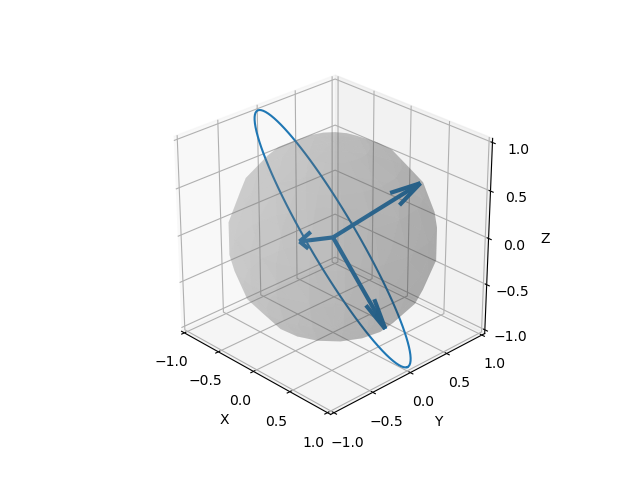
\includegraphics[width=0.8\textwidth]{fig1.png}
            \caption{矩阵$B$的三个特征向量的方向及其二次型}
            \label{fig:1.4}
        \end{figure}

\end{enumerate}

\clearpage

\subsection{正定矩阵(15pt)}
对称矩阵$K$如果满足对于任意非零向量$u$ 都有$u^TKu > 0$,就被称为“正定”矩阵。
\begin{enumerate}[(a)]
    \item (7pt)我们根据矩阵
    $$A = \begin{pNiceMatrix}
        1 &  & & \\ -1 & 1 & & \\ & -1 & 1 & \\ & & -1 & 1 \\ & & & -1
    \end{pNiceMatrix}$$
    构造
    $$K_4 = A^T A = \begin{pNiceMatrix}
        2 & -1 & 0 & 0 \\ -1 & 2 & -1 & 0 \\ 0 & -1 & 2 & -1 \\ 0 & 0 & -1 & 2
    \end{pNiceMatrix}$$
    请证明对于每一个非零向量$u$,都有$u^TK_4u=u^TA^TAu>0$。请先说明为什么$u^TA^TAu\ge 0$,然后说明只能取大于号。
    \item (8pt)对于哪些$b$的取值,这个矩阵$S$是正定的?对于哪些$b$,它是半正定的?它的主元是什么?
\end{enumerate}
\textbf{Solution:}
\begin{enumerate}[(a)]
    \item $u^TK_4u$满足:
    \begin{align*}
        u^TK_4u &= u^TA^TAu \\
                &= (Au)^TAu \ge 0
    \end{align*}
    当且仅当$Au=0$时,等号成立,即$u\neq\vb{0}$,因此$u^TK_4u>0$。
    \item 由正定和半正定的定义,显然$S$的一阶主子式为正,考虑二阶主子式:
    $$\det(S) = 8 - b^2$$
    当$-2\sqrt{2} \ge b \ge 2\sqrt{2}$时,$S$是半正定的;当$-2\sqrt{2} < b < 2\sqrt{2}$时,$S$是正定的。
\end{enumerate}
\end{document}